\chapter{Background}
\section{Refinery}
	Refinery \cite{refinery} is an open-source framework designed to automate the synthesis of diverse, consistent domain-specific graph models. 
	It features a high-level specification language that leverages partial models to concisely define a variety of graph generation challenges. 
	With its modern, cloud-based architecture, Refinery provides a scalable "Graph Solver as a Service" that applies logic-based reasoning rules to 
	efficiently produce diverse solutions by refining partial models. This framework supports applications such as system-level architecture synthesis,
	test generation for modeling tools, and traffic scenario synthesis for autonomous vehicles.

\section{Java}
	Java \cite{java} is a widely-used, object-oriented programming language known for its platform independence, achieved through the Java Virtual Machine (JVM) 
	which allows Java applications to run on any device or operating system. This portability, combined with its robustness, scalability, and extensive libraries,
	makes Java a popular choice for developing enterprise-level applications, web services, and backend systems.

	Java supports core object-oriented programming principles like encapsulation, inheritance, and polymorphism, promoting code modularity and reusability.
	Additionally, Java’s memory management is handled through an automatic garbage collector, which improves performance by reclaiming memory used by objects 
	that are no longer accessible. Java also has a strong emphasis on security, providing a secure runtime environment through features such as bytecode 
	verification and sandboxing, which helps prevent unauthorized access and code manipulation.

\section{Gradle}
	Gradle \cite{gradle} is a build automation tool for multi-language software development. It controls the development process in the tasks of compilation 
	and packaging to testing, deployment, and publishing. Supported languages include Java (as well as Kotlin, Groovy, Scala), C/C++, and JavaScript.
	Gradle builds on the concepts of Apache Ant and Apache Maven, and introduces a Groovy- and Kotlin-based domain-specific language contrasted with 
	the XML-based project configuration used by Maven. Gradle uses a directed acyclic graph to determine the order in which tasks can be run, 
	through providing dependency management. It runs on the Java Virtual Machine.

	Gradle was designed for multi-project builds, which can grow to be large. It operates based on a series of build tasks that can run serially or in parallel.
	Incremental builds are supported by determining the parts of the build tree that are already up to date; any task dependent only on those parts does not need 
	to be re-executed. It also supports caching of build components, potentially across a shared network using the Gradle Build Cache. 
	The software is extensible for new features and programming languages with a plugin subsystem. 

\section{Jetty}
	Eclipse Jetty \cite{jetty} provides a highly scalable and memory-efficient web server and servlet container, supporting many protocols
	 such as HTTP/3,2,1 and WebSocket.

\section{JSON}
	JSON (JavaScript Object Notation) \cite{json} is a lightweight data-interchange format. It is easy for humans to read and write. 
	It is easy for machines to parse and generate. It is based on a subset of the JavaScript Programming Language Standard ECMA-262 3rd Edition - December 1999.
	JSON is a text format that is completely language independent but uses conventions 
	that are familiar to programmers of the C-family of languages, including C, C++, \text{C\#}, Java, JavaScript, Perl, Python, and many others. These properties make JSON an ideal data-interchange language.

	JSON is built on two structures:

	\begin{itemize}
		\item A collection of name/value pairs. In various languages, this is realized as an object, record, struct, dictionary, hash table, 
		keyed list, or associative array.
		\item An ordered list of values. In most languages, this is realized as an array, vector, list, or sequence.
	\end{itemize}

	These are universal data structures. Virtually all modern programming languages support them in one form or another. 
	It makes sense that a data format that is interchangeable with programming languages also be based on these structures.

	In JSON, they take on these forms:

	\begin{itemize}
		\item An object is an unordered set of name/value pairs.
		\item An object begins with left brace and ends with right brace.
		\item Each name is followed by colon and the name/value pairs are separated by comma.
	\end{itemize}

\section{REST API}
	A REST API \cite{restapi} (also called a RESTful API or RESTful web API) is an application programming interface (API) that conforms to the design principles of 
	the representational state transfer (REST) architectural style. REST APIs provide a flexible, lightweight way to integrate applications and to connect 
	components in microservices architectures.

	REST APIs communicate through HTTP requests to perform standard database functions like creating, reading,
	updating and deleting records (also known as CRUD operations) within a resource.

	REST API would use a GET request to retrieve a record. A POST request creates a new record. A PUT request updates a record, and a DELETE request deletes one. 
	All HTTP methods can be used in API calls. A well-designed REST API is similar to a website running in a web browser with built-in HTTP functionality.

\section{Remote Procedure Call}
	In distributed computing, a remote procedure call (RPC) \cite{rpc} is when a computer program causes a procedure (subroutine) to execute in a different address space 
	(commonly on another computer on a shared computer network), which is written as if it were a normal (local) procedure call, without the programmer 
	explicitly writing the details for the remote interaction. That is, the programmer writes essentially the same code whether the subroutine is local to 
	the executing program, or remote.
	This is a form of client–server interaction (caller is client, executor is server), typically implemented via a request–response message passing system.

\section{WebSocket}
	The WebSocket Protocol \cite{websocket} enables two-way communication between a client
	running untrusted code in a controlled environment to a remote host
	that has opted-in to communications from that code.  The security
	model used for this is the origin-based security model commonly used
	by web browsers.  The protocol consists of an opening handshake
	followed by basic message framing, layered over TCP.  The goal of
	this technology is to provide a mechanism for browser-based
	applications that need two-way communication with servers that does
	not rely on opening multiple HTTP connections

	Historically, creating web applications that need bidirectional
	communication between a client and a server (e.g., instant messaging
	and gaming applications) has required an abuse of HTTP to poll the
	server for updates while sending upstream notifications as distinct
	HTTP calls.
	\begin{figure}[h!]
		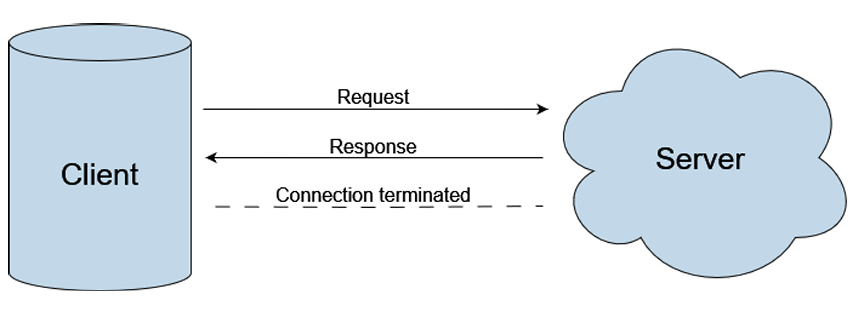
\includegraphics{include/http.PNG}
		\caption{HTTP connection}
	\end{figure}
	This results in a variety of problems:

	\begin{enumerate}
		\item The server is forced to use a number of different underlying TCP
		connections for each client: one for sending information to the
		client and a new one for each incoming message.
		\item The wire protocol has a high overhead, with each client-to-server
		message having an HTTP header.
		\item The client-side script is forced to maintain a mapping from the
		outgoing connections to the incoming connection to track replies.
	\end{enumerate}

	A simpler solution would be to use a single TCP connection for
	traffic in both directions.  This is what the WebSocket Protocol
	provides.

	\begin{figure}
		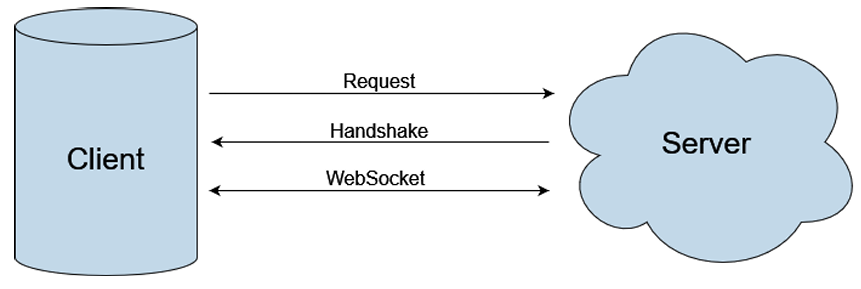
\includegraphics{include/websocket.PNG}
		\caption{WebSocket connection}
	\end{figure}

\section{Shell}
	In computing, a shell \cite{shell} is a computer program that exposes an operating system's services to a human user or other programs. 
	In general, operating system shells use either a command-line interface (CLI) or graphical user interface (GUI), 
	depending on a computer's role and particular operation. It is named a shell because it is the outermost layer around the operating system.

	Operating systems provide various services to their users, including file management, process management (running and terminating applications), batch processing, and operating system monitoring and configuration.

	Most operating system shells are not direct interfaces to the underlying kernel, even if a shell communicates with the user via peripheral devices 
	attached to the computer directly. Shells are actually special applications that use the kernel API in just the same way as it is used by 
	other application programs. A shell manages the user–system interaction by prompting users for input, interpreting their input, and then 
	handling output from the underlying operating system. In addition to shells running on local systems, there are different ways to make remote 
	systems available to local users; such approaches are usually referred to as remote access or remote administration.

\section{Shell script}
	A shell script \cite{shellscript} is a computer program designed to be run by a Unix shell, a command-line interpreter. The various dialects of shell scripts 
	are considered to be command languages. Typical operations performed by shell scripts include file manipulation, program execution, and printing text.
	The term is also used more generally to mean the automated mode of running an operating system shell.

\section{Cloud Computing}
	Cloud computing \cite{cloud} is the on-demand availability of computing resources (such as storage and infrastructure), as services over the internet. 
	It eliminates the need for individuals and businesses to self-manage physical resources themselves, and only pay for what they use.

	Cloud computing service models are based on the concept of sharing on-demand computing resources, software, and information over the internet. 
	Companies or individuals pay to access a virtual pool of shared resources, including compute, storage, and networking services, which are located on
	remote servers that are owned and managed by service providers. 

	One of the many advantages of cloud computing is that you only pay for what you use. This allows organizations to scale faster and more efficiently 
	without the burden of having to buy and maintain their own physical data centers and servers.  
	In simpler terms, cloud computing uses a network (most often, the internet) to connect users to a cloud platform where they request and access 
	rented computing services.

	There are three different cloud computing deployment models:
	\begin{itemize}
		\item \textbf{Public clouds} are run by third-party cloud service providers. They offer compute, storage, and network resources over the internet, 
		enabling companies to access shared on-demand resources based on their unique requirements and business goals.
		The most popular public cloud providers are Amazon, Google and Microsoft.
		\item \textbf{Private clouds} (also known as "on-premises" or "on-prem") are built, managed, and owned by a single organization 
		and privately hosted in their own data centers.
		They provide greater control, security, and management of data while still 
		enabling internal users to benefit from a shared pool of compute, storage, and network resources.
		\item \textbf{Hybrid clouds} are the mixture of using both public- and private clouds within the same organization.
	\end{itemize}

	There are three main types of cloud computing services:
	\begin{itemize}
		\item \textbf{Infrastructure as a service (IaaS)} offers on-demand access to IT infrastructure services, 
		including compute, storage, networking, and virtualization. It provides the highest level of control over your IT 
		resources and most closely resembles traditional on-premises IT resources.
		\item \textbf{Platform as a service (PaaS)} offers all the hardware and software resources needed for cloud 
		application development. With PaaS, companies can focus fully on application development without 
		the burden of managing and maintaining the underlying infrastructure.
		\item \textbf{Software as a service (SaaS)} delivers a full application stack as a service, from underlying 
		infrastructure to maintenance and updates to the app software itself. A SaaS solution is often an end-user application
		, where both the service and the infrastructure is managed and maintained by the cloud service provider.
	\end{itemize}

\subsection{Cloud Native}

\subsection{Scaling}

\subsection{Load Balancing}

\subsection{Amazon-related technologies}
\subsubsection{Amazon Web Services(AWS)}

\subsubsection{Amazon Elastic Compute Cloud (EC2)}

\subsubsection{Amazon Elastic Container Service (ECS)}

\subsubsection{Virtual Private Cloud (VPC)}

\subsubsection{Application Load Balancing (ALB)}

\subsubsection{EC2 Auto Scaling}

\section{Containers}

\subsection{Docker}

\subsection{Docker compose}
